\documentclass[handout]{beamer}
%\usepackage[german]{babel}
\usepackage[utf8x]{inputenc}
\usepackage{listings}

\usetheme{Madrid}
% Other valid themes
%   Antibes, Bergen, Berkeley, Berlin, Copenhagen
%   Darmstadt, Dresden, Frankfurt, Goettingen, Hannover
%   Ilmenau, JuanLesPins, Luebeck, Madrid, Malmoe
%   Marburg, Montpellier, PaloAlto, Pittsburgh, Rochester
%   Singapore, Szeged, Warsaw, boxes, default

%möglich: Antibes, Darmstadt, Frankfurt, Madrid, Montpellier, Singapore

\usecolortheme{dove}
% Other valid color schemes
%    albatross, beaver, beetle, crane, dolphin
%    dove, fly, lily, orchid, rose, seagull
%    seahorse, whale and the one and only wolverine

%möglich: albatross, beaver, dove, whale

\title[Reportbasierte CSP Erzeugung]{Reportbasierte CSP-Erzeugung}
\subtitle{Einführungsvortrag Projektgruppe}
\author[Klaassen]{Malte Klaassen}
%\institute[Kurzform]{Institut}
\date{2016-06-16}

\begin{document}

\begin{frame}%1
\titlepage
\end{frame}

\begin{frame}%2
	\frametitle{Inhaltsverzeichnis}
	\tableofcontents%[pausesections]
\end{frame}

\section{Cross Site Scripting}
\begin{frame}[c]
\frametitle{Cross Site Scripting}
\begin{itemize}
\item Angriff auf Nutzer einer Webseite
\item Einfügen von Skripts in generierten HTML-Code
\item Ermöglicht durch unzureichend geprüfte Eingaben
\begin{itemize}
\item Reflected XSS
\item Persistent XSS
\end{itemize}
\end{itemize}
\end{frame}

\section{Content Security Policy}
\begin{frame}[c]
\frametitle{Content Security Policy}
\begin{itemize}
\item "[...] defines a mechanism by which web developers can control the resources which a particular page can fetch or execute [...]" (CSP Level 3)
\item Server sendet Policy in HTTP-Header Content-Security-Policy
\item Report/Fetch Directives
\item Alternativer Header-Name: Content-Security-Policy-Report-Only
\end{itemize}
\end{frame}

\begin{frame}
\frametitle{Fetch Directives}
\begin{itemize}
\item Für XSS insb. relevant: script-src
\item Directive-Werte:
\begin{itemize}
\item URLs (ohne Dateiname): https://example.com
\item 'none'
\item 'self'
\item 'unsafe-inline'/'unsafe-eval'
\item 'nonce-VALUE' mit VALUE einem base64-String
\item 'HASHALG-VALUE' mit HASHALG einem Hash-Algorithmus, VALUE dem entsprechenden base64-String
\end{itemize}
\item Neu hinzugeladene Scripts müssen i.A. die Policy ebenfalls erfüllen
\end{itemize}
\end{frame}

% Alexa Top 10 mit CSP: 
% Facebook, aber erlaubt unsafe-inline/unsafe-eval
% Twitter, erlaubt unsafe-eval für scripts

\begin{frame}
\frametitle{Policy Beispiel}
\begin{figure}[ht]
	\centering
	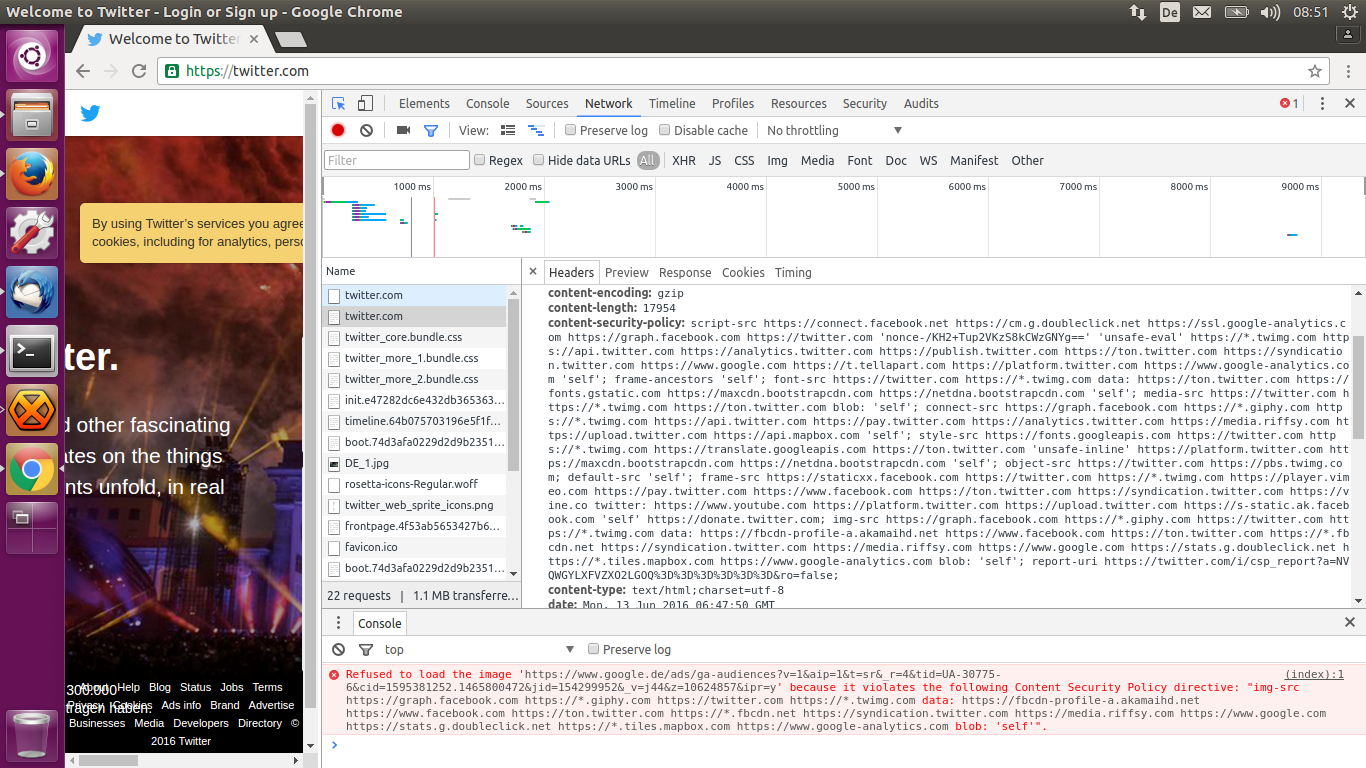
\includegraphics[width=12cm]{twitter_csp.png}
	\caption{CSP-Header twitter.com}
\end{figure}
\end{frame}

\section{Manuelle Policy Erzeugung}
\begin{frame}[c]
\frametitle{Probleme der Policy Erzeugung}
\begin{itemize}
\item Viele verschiedene Ressourcen
\item Betreiber kennt nicht alle Ressourcen
\begin{itemize}
\item Erstellung durch WCMS
\item Einbinden durch Fremdskripte
\end{itemize}
\item Ressourcen ändern sich
\begin{itemize}
\item Inhalte hinzugefügt/entfernt
\item Fremdskripte ändern sich
\end{itemize}
\end{itemize}
\end{frame}

\section{Reportbasierte Policy Erzeugung}
\begin{frame}[c]
\frametitle{Reportbasierte Policy Erzeugung}
\begin{itemize}
\item Ziel: Erstellung von Policies aus Reports, unabhängig vom verwendeten Webserver
\end{itemize}
\end{frame}

\begin{frame}[c]
\frametitle{Policy Erzeugung mit Rückfrage}
\begin{itemize}
\item Sammlung von Reports, Hinzufügen zur Policy nur nach Rückfrage beim Seitenbetreiber
\begin{itemize}
\item Neue Ressourcen müssen erst freigeschaltet werden, sind zuerst nicht verfügbar
\item Bei Einbindung durch fremde Skripte: Betreiber kennt nicht alle validen Ressourcen\\
Kann durch Zurückführung auf ursprüngliche Skripte vereinfacht werden
\item Auwändig/nicht automatisiert
\end{itemize}
\end{itemize}
\end{frame}

\begin{frame}[c]
\frametitle{Policy Erzeugung - Beliebige Quellen}
\begin{itemize}
\item Vollautomatische Generierung der Policy zur Laufzeit aus Violation Reports von beliebigen Quellen
\begin{itemize}
\item Neue Ressourcen sind zuerst nicht verfügbar
\item Bewertung einer Violation/Ressource nichttrivial nur anhand der Häufigkeit möglich \\$\implies$ manipulierbar durch Angreifer
\end{itemize}
\end{itemize}
\end{frame}

\begin{frame}[c]
\frametitle{Policy Erzeugung - Sichere Quellen, Produktionsdaten}
\begin{itemize}
\item Vollautomatische Generierung der Policy aus Violation Reports aus sicheren Quellen auf Produktionsdatensätzen
\begin{itemize}
\item Sichere Quelle : Modul des Proxies, bestehende Tests, ...
\item Quelle muss Kenntnisse über die geproxyte Seite haben
\item Schützt nicht gegen Persistent XSS 
\end{itemize}
\end{itemize}
\end{frame}

\begin{frame}[c]
\frametitle{Policy Erzeugung - Sichere Quellen, Testdaten}
\begin{itemize}
\item Vollautomatische Generierung der Policy aus Violation Reports aus sicheren Quellen auf sicheren Testdatensätzen
\begin{itemize}
\item Kann bestehendes Testsystem nutzen
\item Schützt auch vor Persistent XSS
\item Policy muss bei jeder Änderung der Ressourcen erstellt werden, auch bei Änderung von Fremdressourcen
\end{itemize}
\end{itemize}
\end{frame}

\begin{frame}[c]
\frametitle{Policy Erzeugung - Sichere Quellen, Testdaten}
\begin{figure}[ht]
	\centering
	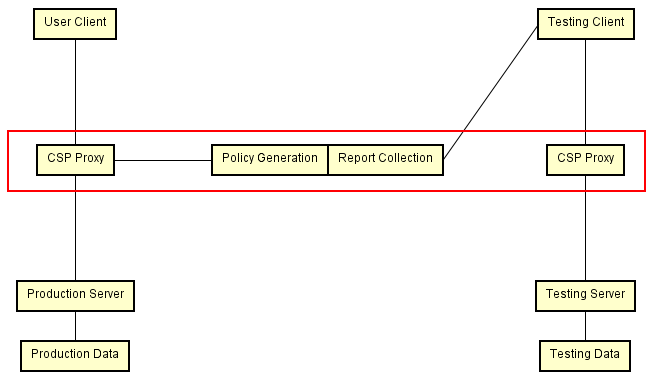
\includegraphics[width=12cm]{schema_2.png}
	%\caption{Testbasierte Erzeugung}
\end{figure}
\end{frame}

\begin{frame}[c]
\frametitle{Policy Erzeugung - Sichere Quellen}
\begin{itemize}
\item Proxy
\begin{itemize}
\item Reverse Proxy, fügt Header hinzu
\item Testing-Header: Erlaube nichts, berichte an Collector
\item Production-Header: Von Generator erzeugte Policy
\end{itemize}
\item Collector
\begin{itemize}
\item Nehme Reports entgegen, gebe diese an Generator weiter
\end{itemize}
\item Generator
\begin{itemize}
\item Nehme Reports vom Collector entgegen, erzeuge Policy
\end{itemize}
\end{itemize}
\end{frame}

\begin{frame}[c]
\end{frame}

\begin{thebibliography}{}
\bibitem[1]{1}
...
\end{thebibliography}



\end{document}

%%% OLD %%%

%\subsection{sub}

%\begin{frame}[c]%24
%\frametitle{Vielen Dank für Ihre Aufmerksamkeit}
%\framesubtitle{Untertitel}
%\begin{itemize}
%\item Ein Item
%\end{itemize}
%\end{frame}
